\section{Pathplanning} 

The first part of the document will lay down the basic concepts and requirements of an oceanography task, focusing on the development of the High Level Controller and a seamless simulator to evaluate the results.

\subsection{Map reading}

The main method of navigation is via GPS and known shoreline database. The ship must be outfitted with proximity sensors later, in order to ensure safe navigation through traffic. During the simulation a reference shore is being generated that simulates a typical fjordic environment: Figure~\ref{fig:linemap}. The map generator is using Random Walk Functions to generate the coastline(s).

\begin{figure}[H]
	\centering
	\includegraphics[width=0.8\textwidth]{img/linemap}
	\caption{The coastlines}
	\label{fig:linemap}
\end{figure}

The generated coastlines are converted to the actual Map, which is a number of surfaces: Figure~\ref{fig:solidmap}.

\begin{figure}[H]
	\centering
	\includegraphics[width=\textwidth]{img/solidmap}
	\caption{The solidified map (the picture shows a north ("upside down") coast)}
	\label{fig:solidmap}
\end{figure}

Reading a solid map is possible from image files as well, using the Python SciPy library

\begin{figure}[H]
	\centering
	\includegraphics[width=0.8\textwidth]{img/worldmap}
	\caption{Image file processed to Map object}
	\label{fig:worldmap}
\end{figure}

\section{Routing}

Upon entering the water, the first task of the vessel in automatic or autonomus mode is to determine the course. Currently the software can not handle rivers, strong wind and magnetic declination, therefore the course is assumed to be identical to the heading.

\paragraph{The Waypoint planner} is responsible for the generating and ordering of the key measurement points. Visiting a set of waypoints on a given map leads to the Traveling Salesman NP-complete problem. Even using dynamic programming, determining the best route with the Held-Karp algorithm the program requires $O(N^2 2^2)$ steps [wiki]. The problem has been in the crosshair of mathematics for a long time, but a fast exact solution has never been found. The waypoint-planning is not time-critical, but a sufficient length of path should be calculated in a reasonable amount of time.

Fortunately the arrangement of the measurement points is relatively dense and predictable, allows only neighboring travels and repeated visits. In order to reach a suitable algorithm, some heuristics of the path planning needs to be examined.
\\

\begin{tcolorbox}[colback=cyan!5,colframe=cyan!40!black,title=Code: Ship.py \\ https://www.dropbox.com/s/fmtsaatql7jqjhw/Ship\texttt{\_}nofilter.py]
\begin{minipage}{0,6\textwidth}
Ship.py implements the Ship Object. Everything related to the handling of a ship is encapsulated in a Ship instance. Multiple instances can be created based on the same object, with different parameters, and they are using the same resources.
\end{minipage}
\begin{minipage}{0,35\textwidth}
\raggedleft
\includegraphics[width=0.8\textwidth]{img/ship}
\end{minipage}
\end{tcolorbox}

\paragraph{In a simple coastline} the points can be placed in a certain order relative to the coast, to achieve a sufficient result. If the shore is relatively smooth, the ship can also travel parallel to the coast, to decrease the required number of turns.

\begin{figure}[H]
	\centering
	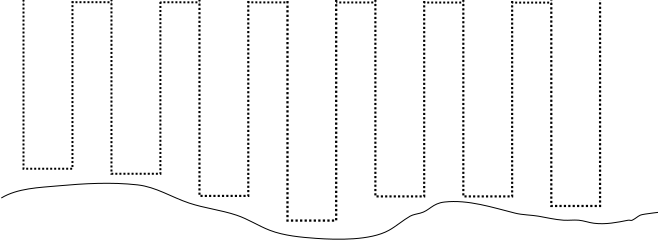
\includegraphics[width=\textwidth]{img/simplecoast}
	\caption{A simple coast and a sufficient path}
	\label{fig:simplecoast}
\end{figure}

\paragraph{Introducing isles and deep bays} to the area complicate the situation. Some waypoints need to be removed, and an avoiding path needs to be taken. This will cause many redundant measurements and very sub-optimal path, if the island density and the complexity of the coast is high.

\begin{figure}[H]
	\centering
	\includegraphics[width=\textwidth]{img/pathislands}
	\caption{Coast with islands}
	\label{fig:pathislands}
\end{figure}

\paragraph{Greedy traversal}

stretches a measurement grid over the area, and the points are traversed in an unpredictable way, using a neirest neighbourgh algorithm.

\begin{figure}[H]
	\centering
	\includegraphics[width=\textwidth]{img/traversal}
	\caption{A random path based on graph traversal}
	\label{fig:traversal}
\end{figure}

 According to [citation] heuristic closest neighbour search is usually 5-10\% worse than the ideal solution. Using the closest neighbour heuristic, the simulation leads to the following path: Figure~\ref{fig:nn}.

\begin{figure}[H]
	\centering
	\includegraphics[width=\textwidth]{img/nn}
	\caption{Neirest neighbourgh algorithm}
	\label{fig:nn}
\end{figure}

\subsection{Lowest cost heuristics}

Even without major nautical engineering skills the following presumption can be made: If there are two paths with identical start and finish and identical lengths (start != finish) the  path with less turning is more effective.
This presumption can be extended to the following theory:

The most effective nautical path between two given points is the one with the least sum cost. The sum cost is the traveled distance times distance cost, plus absolute turnining times turning cost.

\begin{align}
	\Sigma C  = dist*C_{dist} + |turn| * C_{turn}
\end{align}

The cost of the distance and the turning depends on the type of the ship. A large, deep draught cargo ship capable of low speed will have a much higher $\frac{Distance}{Turn}$ cost ratio than a narrow military cruiser.


Using the considerations above a cost based nearest neighbour algorithm is introduced, where the lowest distance is replaced with lowest cost. The algorithm checks every point to determine which is the cheapest destination. To avoid path-loops in the map, the waypoints already visited are stored in a list. If the examined point is already in the list, the cost is increased with a redundancy value, so the algorithm will chose a different, slightly more expensive, but still unvisited measurement point. The algorithm also checks, if the path leading to the examined waypoint is clear of obsticles.

Running the simulation with the above pathplanner results in the following course: Figure~\ref{fig:lc}.

\begin{figure}[H]
	\centering
	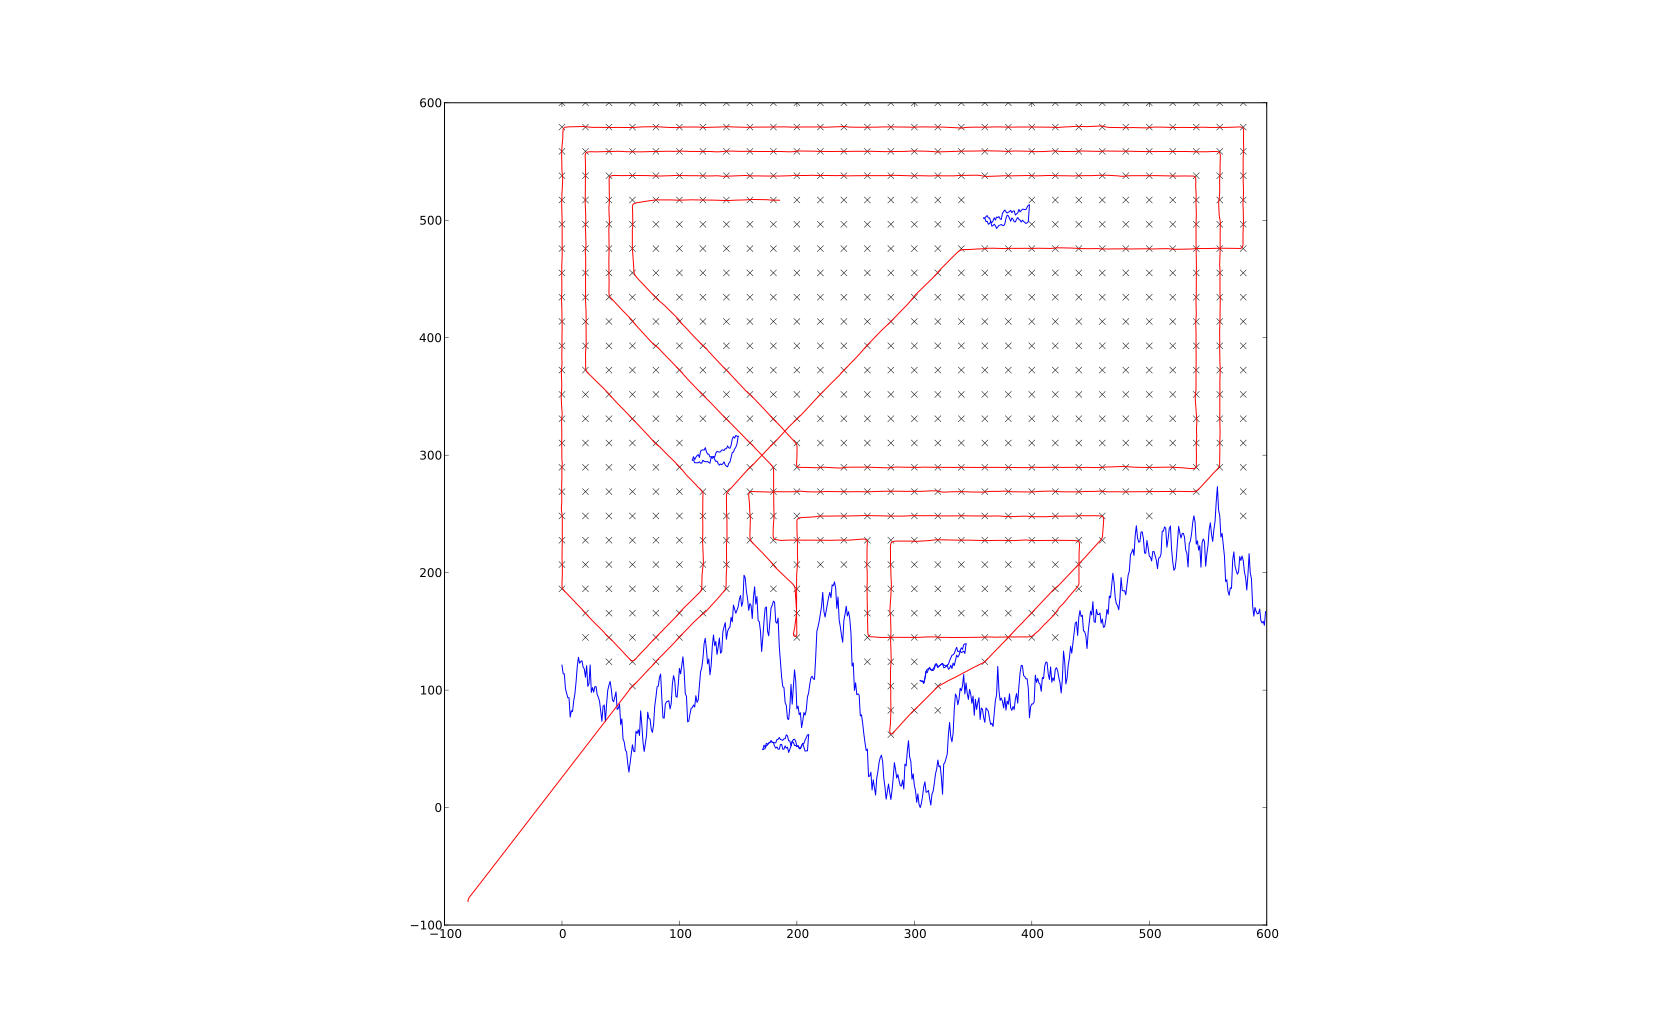
\includegraphics[width=\textwidth]{img/geee}
	\caption{Lowest cost algorithm}
	\label{fig:lc}
\end{figure}

This navigation method works adequatly in open environments. However, if the map is consisted of tight narrows and hard to navigate areas, the algorithm above fails to exit certain areas of the map. To be able to operate in such shores, a different kind of routing is required.

I call this method "Ripple", because the points examined are moving away from the surface vessel in a circular shape (well, in a rectangular actually) like a ripple. The ripple checks every neighbouroing waypoint, that wasnt checked so far, and stores the previous life of the ripple. If a point is found that has not been visited before, a list of waypoints are returned, and the ship will sail through them, and reach the destination.

Figure~\ref{fig:ripple} illustrates this navigation method by simulating a task on the map of the Earth.

\begin{figure}[H]
	\centering
	\includegraphics[width=\textwidth]{img/ripple}
	\caption{Ripple routing algorithm}
	\label{fig:ripple}
\end{figure}

\section{Navigation}

Once the required course has been set, the control system will take over the handling of the ship. The Navigation is the first and highest layer of control in the High Level Controller. In order to explain the navigation, the coordinate systems must be defined first.

\subsection{Frames of reference}

The operator team and the GPS sensor are using the Earth Centered Earth Fixed (ECEF) coordinate systems. Navigation on a spherical surface would introduce a lot of unnecessary calculations in every control cycle, since a plane can be fit onto the surface with minimal error, because the small vessel has limited maximum range.

During the Navigation the North East Down coordinate system is used to determine the attitude and position of the ship. The NED coordinate system is centered to the first GPS measurement coordinate.

A third Body Frame is also defined, the dynamic system of the ship was calculated in this frame.

\begin{figure}[H]
	\centering
	\includegraphics[width=\textwidth]{img/reference_frames}
	\caption{Used coordinate systems}
	\label{fig:coordinatesystem}
\end{figure}

\begin{align}
	\lambda = longitude  \quad \phi = latitude
	\\ GPS_{[\lambda , \phi , h]} \Longleftrightarrow [X_{NED}; Y_{NED}; Z_{NED}]
\end{align}

\subsection{Required heading}

The heading of the ship is defined in NED coordinate system. The required heading is determined by the Law of Cosines, based on the Position of the Ship and the Position of the next Sub-Waypoint.
\begin{center}
\includegraphics[scale = 0.4]{img/Law_of_Cosines}
\end{center}
Problems rise and corrections are necessary, if the heading of the ship $\theta$ is $\theta < -\pi$ or $\theta < \pi$. The heading of the ship is calculated based on the Gyro sensor and the heading can have any value in the form of: 
\begin{align}
\theta = [-{\pi} ; \pi ] \pm 2 \cdot k \cdot \pi
\end{align}\\

\begin{tcolorbox}[colback=cyan!5,colframe=cyan!40!black,title=Code: FunctionLibrary.py \\ https://www.dropbox.com/s/7nx7helisvss21a/FunctionLibrary.py]
\begin{minipage}{0,6\textwidth}
Some functions required by the software are general parametric mathematical functions, which can not be connected to any object. These functions, like the Law of Cosines, and the distance calculator function can be found in the Function Library.
\end{minipage}
\begin{minipage}{0,35\textwidth}
\raggedleft
\includegraphics[width=0.8\textwidth]{img/functionlibrary}
\end{minipage}


\end{tcolorbox}

Before invoking the control procedure, all of the heading angles must be transformed into the $[-\pi ; \pi]$ interval.
This procedure causes a possible error though.

\includegraphics[width=\textwidth]{img/Headings}

The required heading or the heading of the ship must be transformed into a different representation, where 
\begin{align}
|\theta_{r}-\theta| < \pi
\end{align}
To keep a consistent heading representation, first the deviation angle 
\begin{align}
\theta = \pi_{r}-\pi
\end{align} is calculated, than transformed to the $[-\pi;\pi]$ interval and finally, with $\delta$ we can transform $\theta_{r}$ to 
\begin{align}
\theta_{r}(\theta) = \theta + \delta
\end{align}
If the conditions above are met, $\theta$ and $\theta_r(\theta)$ will always yield values that result in correct controller output.

\section{Simulator}
In order to test the generated path and eliminate some hazards of potential design errors or malfunctions, a seamless simulator is required that simulates the behaviors of the ship. \\

\begin{tcolorbox}[colback=cyan!5,colframe=cyan!40!black,title=Code: Simulator.py \\ https://www.dropbox.com/s/agron9anslev6xw/Simulator.py]
\begin{minipage}{0,6\textwidth}
According to the guidelines of the seamless simulator, this part of the system has its own distinctive object. Everything related to the simulator and everything that is unknown during the mission is stored and handled here.
\end{minipage}
\begin{minipage}{0,35\textwidth}
\raggedleft
\includegraphics[width=0.8\textwidth]{img/simulatorcode}
\end{minipage}
\end{tcolorbox}

\subsection{Requirements of the simulator}

The simulator developed for the project must meet the following conditions, otherwise the simulation might return false results, misguiding the whole development process.
\begin{itemize}
	\item The software controlling the simulated system must be unaware of the simulation
	\item The control software must be completely independent of the simulator, its variables and its functions
	\item The control software can communicate only through the same channel, as it would during normal operation
	\item Any parameters and states that are not known, only measured (e.g.: measured position != actual position) must be stored in the simulator, and must not be accessed directly from the control software
\end{itemize}

To fulfill the requirements above, the following simulator has been implemented:

\begin{figure}[H]
	\centering
	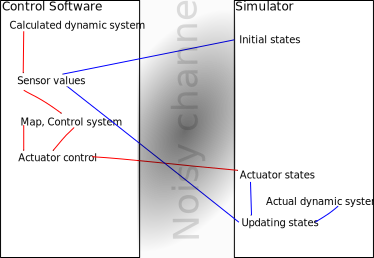
\includegraphics[width=\textwidth]{img/simulator}
	\caption{System simulator}
	\label{fig:simulator}
\end{figure}